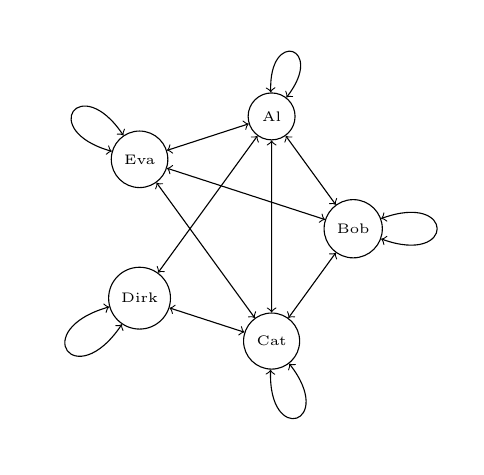
\begin{tikzpicture}[scale=1.5]
    \node[circle, draw] (a1) at (72:1) {\tiny Al};
    \node[circle, draw] (a2) at (0:1) {\tiny Bob};
    \node[circle, draw] (a3) at (-72:1) {\tiny Cat};
    \node[circle, draw] (a4) at (-144:1) {\tiny Dirk};
    \node[circle, draw] (a5) at (144:1) {\tiny Eva};
    \foreach \i in {1,...,5}
    \draw[<->] (a\i) edge [in=164-\i*72, out=124-\i*72,looseness=10] (a\i);
  
    \draw[<->] (a2) edge (a1);
    \draw[<->] (a3) edge (a1);
    \draw[<->] (a4) edge (a1);
    \draw[<->] (a5) edge (a1);
    \draw[<->] (a3) edge (a2);
    \draw[<->] (a5) edge (a2);
    \draw[<->] (a4) edge (a3);
    \draw[<->] (a5) edge (a3);
  \end{tikzpicture}